\chapter{Theoretische Einführung}



\section{Grundlagen des 3D-Drucks mittels selektivem Laserschmelzen (SLM)}
	Die \emph{additive Fertigung} (AM) spielt in unserem Leben eine immer größere Rolle. Während
	sich bereits ein Hobbymarkt für preisgünstige 3D-Drucker im eigenen Haushalt etabliert hat, ist
	die industrielle Anwendung nicht zu vernachlässigen. Eine von Essentium, einem Hersteller von
	industriellen 3D-Druckern und Materialien, angefertigte Umfrage zeigte, dass sich die Anzahl der
	Firmen, die 3D-Druck zur industriellen Fertigung benutzen, von 2018 auf 2019 fast verdoppelte.
	Während der Anteil 2018 noch bei 21\% lag, änderte er sich innerhalb eines Jahres auf 40\%
	\cite{stevenson2019survey}.

	Obwohl es eine Vielzahl unterschiedlicher Methoden der additiven Fertigung gibt, funktionieren
	allen Methoden nach einem ähnlichen Grundprinzip: Das digitale 3-dimension\-ale Objekt wird durch
	einen sogenannten \emph{Slicer} in Schnittebenen unterteilt, die vom 3D-Drucker nacheinander
	produziert und aufgeschichtet werden.

	\subsection{Funktionsweise und Unterschiede zu anderen Methoden}
		Das vermutlich bekannteste Verfahren zur additiven Fertigung ist wahrscheinlich das
		\emph{Fused Depositing Modeling} (FDM), aus markenrechtsgründen auch bekannt als
		\emph{Fused Filament Fabrication} (FFF). Dabei wird ein Kunststofffilament aufgeschmolzen
		und durch eine Düse extrudiert. Die Düse (\emph{Hotend}) fährt hierbei wie in Abbildung
		\ref{fig:fdm} dargstestellt die Schnittebene ab, sodass Ebene für Ebene das gewünschte
		Objekt aufgeschichtet wird. Schichtdicken sind bei diesem Verfahren üblicherweise zwischen
		\SI{0,025}{\milli\meter} und \SI{1,25}{\milli\meter} \cite{wikipedia2021fused}.

		Obwohl dieses Verfahren relativ einfach umzusetzen ist wird es durch verschiedene Faktoren
		limitiert. So ist beispielsweise für die Qualität die Form des zu druckenden Objekts relevant.
		Außerdem ist dieses Verfahren auf formbare Materialien beschränkt, wie Thermoplaste und
		Formwachse \cite{wikipedia2021fused}.

		\begin{figure}[ht]
			\centering
			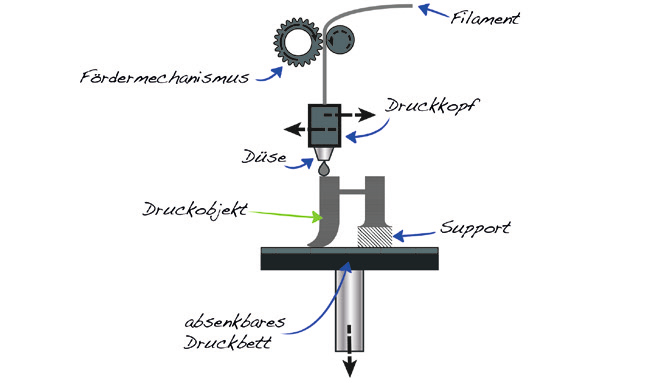
\includegraphics[width=\textwidth]{chapter/main/img/FDM.png}
			\caption[Schematische Darstellung des FDM-/FFF-Verfahrens]{Schematische Darstellung
			einer möglichen Konfiguration des als FDM oder FFF bekannten 3D-Druck-Verfahrens.
			Ein Fördermechanismus schiebt das Filament durch eine aufgeheizte Düse. Durch eine
			Bewegung der Düse und/oder des Druckbetts in mindestens 3 Achsen erfolgt eine Formung
			des Objektes Ebene für Ebene. \cite[S. 114]{horsch20143d}}
			\label{fig:fdm}
		\end{figure}

		Das in dieser Arbeit beobachtete Verfahren ist jedoch das \emph{selektive Laserschmelzen}
		(SLM). Der Drucker besteht hierbei aus zwei Gefäßen mit beweglichen Böden (Abbildung
		\ref{fig:slm_sls}). Das Gefäß für den Materialvorrat ist mit dem Material in Pulverform
		gefüllt, während das andere wenig bis gar nicht gefüllt ist. Beim Drucken einer neuen Ebene
		hebt sich der Boden des Materialvorrats und eine Walze (\emph{Beschichtungseinheit}) überträgt
		das dosierte Material in den den Druckraum, dessen Druckbett abgesenkt wird. Ein beweglicher
		Laser fährt nun die gewünschte Schnittebene ab und verschmilzt das Pulver zu einer festen Form.

		\begin{figure}[ht]
			\centering
			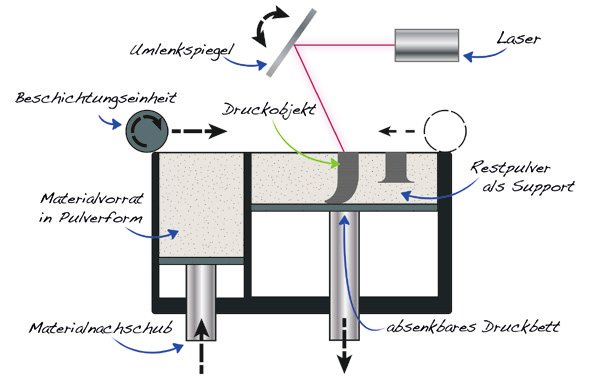
\includegraphics[width=\textwidth]{chapter/main/img/SLS_SLM.png}
			\caption[Schematische Darstellung des SLM-Verfahrens]{Schematische Darstellung
			des SLM-Verfahrens. Der bewegliche Spiegel sorgt für eine präzise Positionierung
			des Laser-Punktes. Während sich der Boden des Vorrats\-gefäßes im Prozess anhebt,
			senkt sich der Boden des Druckraums ab. \cite[S. 119]{horsch20143d}}
			\label{fig:slm_sls}
		\end{figure}

	\subsection{Einfluss der Lasergeschwindigkeit auf die Oberflächenbeschaffenheit}
	\subsection{Beobachtbare Defekte im Material}


\section{Molekulardynamische Modellierung von SLM}
	\subsection{Grundlegende Funktionsweise der Molekulardynamik (MD)}
	\subsection{Notwendige Näherungen und Vereinfachungen}
		\todo[color=red]{Kleinere Skala und größere Gravitation mithilfe von \cite{glosli2007extending} motivieren.}
	\subsection{Implementierung des Laser}
	\subsection{Besonderheiten bei der Simulationssoftware IMD}
